% !TeX root = ../praktikum.tex
% !TeX encoding = UTF-8
% !Tex spellcheck = de_DE

Im folgendem Abschnitt wurden die Messungen des vorigen Versuchsteils im Wesentlichen wiederholt, mit dem Unterschied, dass anstatt eines Gleichstroms ein Wechselstrom die Probe durchfließt. 
%mit $U_{RMS}=\unit[1]{V}$ angelegt wurde und ein \unit[9,95]{$M\Omega$} Widerstand in Reihe geschaltet wurde.  Um einen Wechselstrom erzeugen zu können, wurden sogenannte Lock-in Verstärker genutzt. Ein Lock-in Verstärker enthält einen Funktionsgenerator, welcher anhand einer einstellbaren Frequenz eine sinusförmige Wechselspannung mit $U_{RMS}=\unit[1]{V}$ ausgibt. 
Dieser wurde mit einem Funktionsgenerator mit der Amplitude $U_{RMS}=\unit[10]{V}$ erzeugt. Um den Strom unabhängig von dem Widerstand des Hall-Streifens zu halten, musste ein hinreichend großer Widerstand in Reihe geschaltet werden. Da der Eigenwiderstand des Hall-Streifens bei einigen Kiloohm lag, wurde ein \unit[9,95]{$M\Omega$} Widerstand verwendet. So kann in guter Näherung angenommen werden, dass der Strom allein durch den zusätzlich angelegten Vorwiderstand zu $I=\nicefrac{U}{R}=\nicefrac{\unit[10]{V}}{\unit[9,95]{M\Omega}}=\unit[1,005]{\mu A}$ bestimmt wurde. Um die kleinen, dennoch auftretenden Schwankungen auszugleichen, wurde der Strom ebenfalls für jeden Datenpunkt aufgezeichnet. Die Berechnung des Widerstandes mit den Formeln~\eqref{eq:rho_xx} und \eqref{eq:rho_xy} wurde entsprechend zeilenweise mit dem gemessenen Strom durchgeführt.

Die verwendeten Messgeräte für die Längs- und Querspannungen wurden mit dem Frequenzgenerator als Referenz verbunden. %TODO: Erklärung
\\

Die aus den Messwerten gewonnen Widerstandswerte sind für die gesamte Magnetfeldreichweite bei maximaler Magnetfeldrampe in Abbildung~\ref{fig:full_range_ac} und für den detaillierten Ausschnitt in Abbildung~\ref{fig:2T_range_ac} aufgetragen.

\begin{figure}[h]
	\centering
	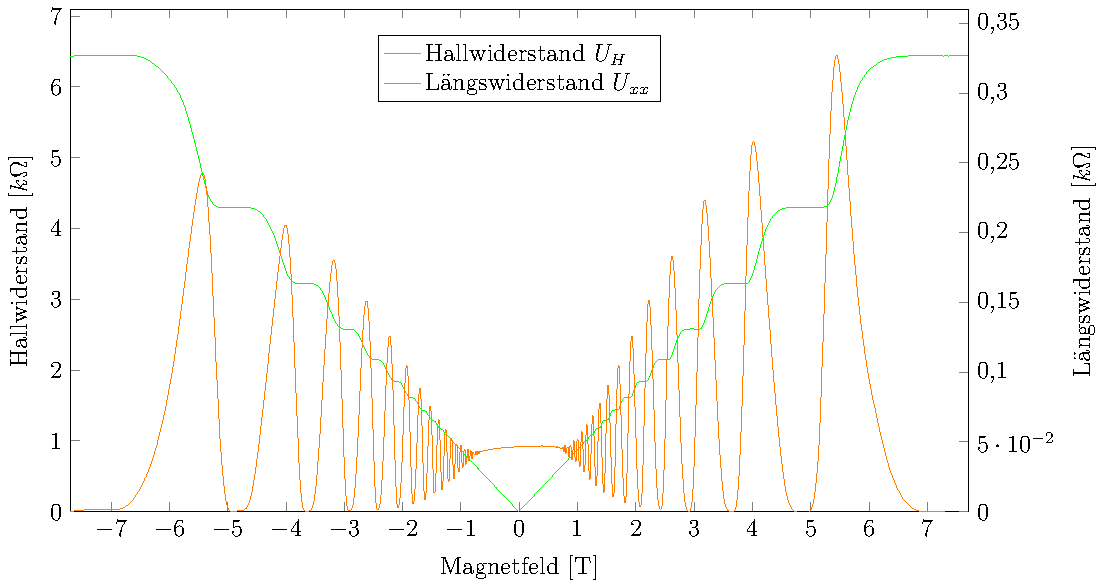
\includegraphics{graphs/ac/full_range.pdf}
	\caption[Wechselstrommessung im maximalen Magnetfeldbereich]{
		Plot des aus den gemessenen Längs- und Querspannungen berechneten Widerständen eines mit Wechselstrom durchflossenen 2DES im maximalen Magnetfeldbereich und maximaler Magnetfeldrampe. Die Hall-Spannung und somit der berechnete Hall-Widerstand nimmt bei negativen Magnetfeldern negative Werte an, Aus Platzgründen wurde diese jedoch in den positiven Bereich geklappt.
	}
	\label{fig:full_range_ac}
\end{figure}

Auch bei diesen Messungen ist die Asymmetrie des positiven und negativen Magnetfeldes zu beobachten. Die


\begin{figure}[h]
	\centering
	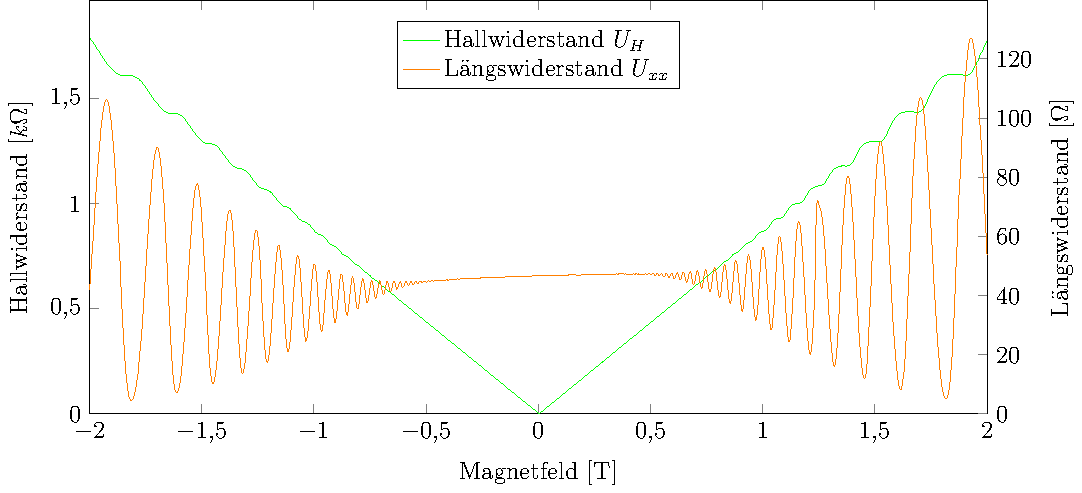
\includegraphics{graphs/ac/pm2T_range.pdf}
	\caption[Höher aufgelöste Gleichstrommessung in Magnetfeldteilbereich]{
		lot des aus den gemessenen Längs- und Querspannungen berechneten Widerständen eines mit Wechselstrom durchflossenen 2DES im reduzierten Magnetfeldbereich und geringerer Magnetfeldrampe. Die Hall-Spannung und somit der berechnete Hall-Widerstand nimmt bei negativen Magnetfeldern negative Werte an, Aus Platzgründen wurde diese jedoch in den positiven Bereich geklappt.
	}
	\label{fig:2T_range_ac}
\end{figure}

